\documentclass[14pt]{extarticle}
\usepackage[utf8]{inputenc}
\usepackage[T1]{fontenc}
\usepackage[spanish,es-lcroman]{babel}
\usepackage{amsmath}
\usepackage{amsthm}
\usepackage{physics}
\usepackage{tikz}
\usepackage{float}
\usepackage{cancel}
\usepackage[autostyle,spanish=mexican]{csquotes}
\usepackage[per-mode=symbol]{siunitx}
\usepackage{gensymb}
\usepackage{multicol}
\usepackage{enumitem}
\usepackage{stackengine}
\usepackage{stix}
\usepackage[left=2.00cm, right=2.00cm, top=2.00cm, 
     bottom=2.00cm]{geometry}

\usepackage{Estilos/ColoresLatex}
\usepackage{makecell}

\newcommand{\textocolor}[2]{\textbf{\textcolor{#1}{#2}}}
%\renewcommand{\questionlabel}{\thequestion)}

\newcommand{\Cancel}[2][black]{{\color{#1}\cancel{\color{black}#2}}}

\newcommand\deci[1]{%
    \kern-.4ex\stackunder[0.4pt]{$#1$}{$\color{blue}\acwunderarcarrow$}
}

\newcommand\decposl[1]{%    <--- Decimal position to left
    \kern-.4ex\stackunder[0.4pt]{$#1$}{%
      \reflectbox{$\color{red}\kern-.6ex\acwunderarcarrow$}
      }
}

\decimalpoint
\sisetup{bracket-numbers = false}

\title{\vspace*{-2cm} Guía de estudio 1er. examen parcial\\  Física III}
\author{M. en C. Ramón Gustavo Contreras Mayén \\ {\fontsize{14}{14}\selectfont Universidad del Valle de México. Campus San Rafael}}
% \institute{Universidad del Valle de México. Campus San Rafael.}
\date{}

\begin{document}
\maketitle

\section*{¿Qué es la física?}

La Física es una ciencia basada en las \textocolor{cobalt}{observaciones} y \textocolor{cadmiumgreen}{medidas} de los fenómenos físicos. La física es una ciencia experimental.
\\
Los físicos observan los fenómenos naturales e intentan encontrar los patrones y principios que los describen. Tales patrones se denominan \textocolor{byzantine}{teorías físicas}  o, si están muy bien establecidos y se usan ampliamente, \textocolor{cordovan}{leyes o principios físicos}.


\section{Conceptos importantes.}

\begin{enumerate}
\item Medición: Es \textocolor{lava}{comparar} una magnitud con otra de la misma especie, llamada patrón.
\item Magnitud: Es una \textocolor{red}{cantidad medible} de un sistema físico a la que se le pueden asignar distintos valores como resultado de una medición o una relación de medidas.
\item Unidad: Es una \textocolor{bole}{cantidad de una determinada magnitud física}, definida y adoptada por convención o por ley. Cualquier valor de una cantidad física puede expresarse como un múltiplo de la unidad de medida.
\end{enumerate}

\subsection{Unidades fundamentales.}

Las \textocolor{airforceblue}{unidades fundamentales} del \textocolor{awesome}{Sistema Internacional de Unidades} (SI), son magnitudes físicas básicas que pueden medirse y son independientes de todas las demás.
\begin{table}[H]
\renewcommand{\arraystretch}{1.1}
\centering
\begin{tabular}{l | c | c}
Magnitud & Unidad & Símbolo \\ \hline 
Longitud & metro & \unit{m} \\ \hline 
Masa & kilogramo & \unit{\kilo\gram} \\ \hline
Tiempo & segundo & \unit{\second} \\ \hline
Temperatura & Kelvin & \unit{\kelvin} \\ \hline
Intensidad eléctrica & Ampere & \unit{\ampere} \\ \hline
Intensidad luminosa & candela & cd \\ \hline
Cantidad de sustancia & mol & \unit{mol}\\ \hline
\end{tabular}
\end{table}

\subsection{Unidades derivadas.}

Son las unidades que provienen de una combinación de las unidades fundamentales.
\begin{table}[H]
\renewcommand{\arraystretch}{1.1}
\centering
\begin{tabular}{l | c | c | c}
Magnitud & Unidad & Símbolo & Equivalencia\\ \hline 
Área & \makecell{metro \\ cuadrado} & \unit{\square\meter} &  \\ \hline
Volumen & \makecell{metro \\ cúbico} & \unit{\cubic\meter} &  \\ \hline
Velocidad & \makecell{metro \\ por segundo} & \unit{\meter\per\second} & \\ \hline
Fuerza & newton & \unit{\newton} & $\displaystyle \unit[per-mode=fraction]{\kilo\gram\meter\per\square\second} $\\ \hline 
Presión & Pascal & \unit{\pascal} & $\displaystyle \unit[per-mode=fraction]{\newton\per\square\meter}$ \\ \hline 
Trabajo & Joule & \unit{\joule} & $\displaystyle \unit[per-mode=fraction]{\newton\meter}$ \\ \hline
\end{tabular}
\end{table}


\section{Tipos de cantidades.}

\begin{enumerate}
\item Cantidad escalar: Es la que queda definida con solo indicar su cantidad en \textocolor{amethyst}{número y unidad de medida}.
\\
Ejemplos: \SI{5}{\kilo\gram},  \SI{20}{\degreeCelsius},  \SI{250}{\square\meter},  \SI{40}{\milli\gram}
\item Cantidad vectorial: Es la que además de definir cantidad en número y unidad de medida, se requiere indicar la dirección y sentido en que actúan.

Se representan de manera gráfica por \textocolor{ao(english)}{vectores},  los cuales deben tener: \textocolor{blue}{magnitud},  \textocolor{red}{dirección}  y \textocolor{cadmiumorange}{sentido}.
\end{enumerate}

\section{Manejando unidades.}

\subsection{Los prefijos de unidades.}

Una vez definidas las unidades fundamentales, es fácil introducir unidades más grande y más pequeñas para las mismas cantidades físicas.

En el sistema métrico, estas otras unidades siempre se relacionan con las fundamentales por múltiplos y submúltiplos de $10$.

\begin{table}[H]
\renewcommand{\arraystretch}{1}
\centering
\begin{tabular}{c | c | c}
Potencia & Prefijo & Abreviatura \\ \hline
\num{d3} & kilo & k \\ \hline
\num{d6} & mega & M \\ \hline
\num{d9} & giga & G \\ \hline
\num{d12} & tera & T \\ \hline
\num{d15} & peta & P \\ \hline
\num{d18} & exa & E \\ \hline
\end{tabular}
\caption{Múltiplos de $10$}
\end{table}

\begin{table}[H]
\renewcommand{\arraystretch}{1}
\centering
\begin{tabular}{c | c | c}
Potencia & Prefijo & Abreviatura \\ \hline
\num{d-1} & deca & d \\ \hline
\num{d-2} & centi & c \\ \hline
\num{d-3} & mili & m \\ \hline
\num{d-6} & micro & $\mu$ \\ \hline
\num{d-9} & nano & n \\ \hline
\num{d-12} & pico & p \\ \hline
\end{tabular}
\caption{Submúltiplos de $10$}
\end{table}


\section{Conversión de unidades.}

En ocasiones se va a requerir expresar una cantidad en términos de otras unidades, ya sea por conveniencia o por que se requiere mantener un manejo homogéneo.

La regla básica es muy sencilla:  utilizar ya sea un \textocolor{blue}{factor de conversión}, o los factores de conversión necesarios.

Estos factores de conversión \enquote{ajustan} las unidades, dejando entonces un problema de tipo aritmético,  es decir, donde tenemos que hacer multiplicaciones o divisiones.

El factor de conversión es un \enquote{uno} que manejamos de manera conveniente.


\subsection{Ejercicio 1.}

Consideremos el siguiente problema: Convertir 100 km a metros.
\par
Siempre será necesario contar de manera previa con el(los) factor(es) de conversión:
\begin{align*}
\SI{1}{\kilo\meter} = \SI{1000}{\meter}
\end{align*}

Procedemos a escribir el valor inicial que se multiplicará por el factor de conversión:
\begin{eqnarray*}
\begin{aligned}
\num{100} \, {\Cancel[red]{\unit{\kilo\meter}}}  \left( \dfrac{\SI{1000}{\meter}}{\num{1} \, \Cancel[red]{\unit{\kilo\meter}}} \right) =  \SI{100000}{\meter}
\end{aligned}
\end{eqnarray*}
Revisa que las unidades \unit{\kilo\meter} en la cantidad inicial están en el numerador, por lo que en el factor de conversión, deberá estar en el denominador, la equivalencia de las unidades, para que de esa manera se cancelen las mismas unidades, es decir:
\begin{align*}
\dfrac{\Cancel{\unit{\kilo\meter}}}{\Cancel{\unit{\kilo\meter}}}
\end{align*}
Las unidades que no quedan con la marca de cancelación, son las unidades en las que reportarmos nuestro resultado. Esta regla de cancelación se debe de anotar con cuidado, ya que dependiendo de la conversión, en el factor de conversión podrá estar en el denominador o en el numerador.

\subsection{Ejercicio 2.}

Ahora consideremos el siguiente problema: Convertir \SI{250}{\kilo\meter\per\hour} a \unit{\meter\per\second}.

Los factores de conversión son:
\begin{eqnarray*}
\begin{aligned}
\SI{1}{\kilo\meter} &= \SI{1000}{\meter} \\[0.5em] 
\SI{1}{\hour} &= \SI{3600}{\second}
\end{aligned}
\end{eqnarray*}

Realizando la conversión:
\begin{eqnarray*}
\begin{aligned}
\num{250} \dfrac{\Cancel[red]{\unit{\kilo\meter}}}{\Cancel[ao]{\unit{\hour}}}  &\left( \dfrac{\SI{1000}{\meter}}{\num{1} \, \Cancel[red]{\unit{\kilo\meter}}} \right)  \left( \dfrac{\num{1} \, \Cancel[ao]{\unit{\hour}}}{\SI{3600}{\second}} \right) =  \dfrac{\SI{250000}{\meter}}{\SI{3600}{\second}} = \\[0.5em] 
&= \SI[per-mode=fraction]{69.44}{\meter\per\second}
\end{aligned}
\end{eqnarray*}

\subsection{Otro ejercicio - Volumen.}
Convertir $7$ galones a \unit{\cubic\centi\meter}.

Los factores de conversión son:
\begin{align*}
1 \, \text{galón} &= \SI{3.785}{\liter} \\[0.5em]
\SI{1}{\liter} &= \SI{1000}{\cubic\centi\meter}
\end{align*}

En este caso identificamos que se tiene que usar un factor de conversión \enquote{intermedio}, ya que no hay un factor de conversión directo. Realizando la conversión:
\begin{eqnarray*}
\begin{aligned}
7 \, \text{\Cancel{ga}}  \left( \dfrac{\num{3.785} \, \Cancel[red]{\unit{\liter}}}{1 \, \text{\Cancel{ga}}} \right)  \left( \dfrac{\SI{1000}{\cubic\centi\meter}}{\num{1} \, \Cancel[red]{\unit{\liter}}} \right) =  \SI{26945}{\cubic\centi\meter}
\end{aligned}
\end{eqnarray*}

\subsection{Siguiente ejercicio de volumen.}

Convertir \SI{96500}{\cubic\centi\meter\per\minute} a  galones/s

\vspace*{0.5cm}
Listamos los factores de conversión:
\begin{eqnarray*}
\begin{aligned}
1 \, \text{ga} &= \SI{3.785}{\liter} \\[0.5em] 
\SI{1}{\liter} &= \SI{1000}{\cubic\centi\meter} \\[0.5em] 
\SI{1}{\minute} &= \SI{60}{\second}
\end{aligned}
\end{eqnarray*}

Notemos que habrá ejercicios en donde se requiera de hacer uso de varios factores de conversión, para que de esa manera se llegue a las unidades que se nos piden en el enunciado. Realizando la conversión:
\begin{eqnarray*}
\begin{aligned}
&\SI[per-mode=fraction]{96500}{\cubic\centi\meter\per\minute}   \left( \dfrac{\SI{1}{\liter}}{\SI{1000}{\cubic\centi\meter}} \right)  \left( \dfrac{1 \, \text{ga}}{\SI{3.785}{\liter}} \right)  \left(  \dfrac{\SI{1}{\minute}}{\SI{60}{\second}} \right) = \\[1em] 
&= \dfrac{96500 \, \text{ga}}{\SI{227100}{\second}} = \\[1em] 
&= 0.424 \dfrac{\text{ga}}{\unit{\second}}
\end{aligned}
\end{eqnarray*}

\subsection{Ejercicio de construcción.}

Convertir \SI{10}{\cubic\meter} a pies${}^{3}$.

\vspace*{0.5cm}
Cuando tenemos unidades que estén elevadas al cuadrado o al cubo, los factores de conversión como tal no se cuentan de manera directa, por lo que hay que construirlos, el procedimiento es sencillo, ya que partimos de un primer factor de conversión, que propiamente es una igualdad. Recordemos que si modifico el lado izquierdo de una igualdad, para que se conserve, debemos de aplicar la misma operación al lado derecho de la igualdad.

El factor de conversión es:
\begin{align*}
1 \, \text{pie} = \SI{0.3048}{\meter}
\end{align*}

El siguiente paso será elevar al cubo ambos lados de la igualdad, así llegaremos a un factor de conversión que involucre el cubo en ambos lados de la igualdad:
\begin{eqnarray*}
\begin{aligned}
1 \, \text{pie} &= \SI{0.3048}{\meter} \\[1em] 
(1 \, \text{pie})^{3} &= (\SI{0.3048}{\meter})^{3}  \hspace{0.2cm} \Rightarrow \hspace{0.2cm} 1 \, \text{pie}^{3} = \SI{0.02831}{\cubic\meter}
\end{aligned}
\end{eqnarray*}

Una vez conocido el factor de conversión, ya se puede utilizar con la cantidad y unidades iniciales:
\begin{align*}
\SI{10}{\cubic\meter}  &\left( \dfrac{1 \, \text{pie}}{\SI{0.02831}{\cubic\meter}} \right) =  353.23 \, \text{pie}^{3}
\end{align*}

\section{Notación científica.}

En muchas ocasiones vemos escritas o escuchamos hablar de cantidades demasiado grandes o muy pequeñas. Para simplificarlas, se utiliza la \textbf{notación científica}. 
\par
La notación científica nos permite escribir grandes o pequeñas cantidades en forma abreviada con potencias de $10$, siguiendo el formato:
\begin{align*}
a.b \times 10^{n}
\end{align*}
donde:
\begin{itemize}
\item $a$ es un dígito.
\item $b$ puede ser un dígito o un conjunto de dígitos.
\item $n$ es el exponente al que se debe elevar la base $10$, puede ser positivo o negativo.
\end{itemize}
Cuando el exponente $n$ sea positivo, nos indica que la cantidad es mayor que la unidad $1$:
\begin{align*}
\num{d1} &= 10 \\
\num{d2} &= 100 \\
\num{d3} &= 1000 \\
\num{d4} &= 10000 \\
\vdots
\end{align*}
Mientras que un exponente negativo $n$, nos dice que la cantidad es menor que la $1$.
\begin{align*}
\num{d-1} &= \dfrac{1}{10} = 0.1 \\[0.5em]
\num{d-2} &= \dfrac{1}{10^{2}} = \dfrac{1}{100} = 0.01 \\[0.5em]
\num{d-3} &= \dfrac{1}{10^{3}} = \dfrac{1}{1000} = 0.001 \\[0.5em]
\num{d-4} &= \dfrac{1}{10^{4}} = \dfrac{1}{10000} = 0.0001 \\[0.5em]
\vdots
\end{align*}

\subsection{Conversión de notación decimal a científica.}

Para representar en notación científica un número menor a la unidad, \textocolor{ao}{el punto decimal se recorre a la derecha} y la exponente de la base $10$ es negativo; el exponente es el número de lugares que se recorrió el punto decimal.

\begin{align*}
0.000156 &= 0 \, \underbrace{\deci{0} \deci{0} \deci{0} \deci{1}.}_{4 \, \text{posiciones}} 56 = \num{1.56d-4} \\[0.5em]
0.0000982 &= 0 \, \underbrace{\deci{0} \deci{0} \deci{0} \deci{0} \deci{9}.}_{5 \, \text{posiciones}} 82 = \num{9.82d-5}
\end{align*}

Para representar en notación científica un número mayor que $1$ o con muchos ceros, el \textocolor{red}{punto decimal} (que no se escribe, pero está hasta la derecha de la cantidad) \textocolor{red}{se recorre a la izquierda} tantos lugares como indica la potencia y el exponente queda positivo.
\begin{align*}
30000 &= 3 \,  \underbrace{\decposl{0} \decposl{0} \decposl{0} \decposl{0}}_{4 \, \text{posiciones}} = \num{3d4} \\[0.5em]
4500000 &= 4. \, \underbrace{\decposl{5} \decposl{0} \decposl{0} \decposl{0} \decposl{0} \decposl{0}}_{6 \, \text{posiciones}} = \num{4.5d6}
\end{align*}

\subsection{Conversión de notación científica a decimal.}

Para pasar un número de notación científica a decimal, si el exponente de la base $10$ es negativo, el punto se recorre a la izquierda y se agregan ceros a la izquierda.
\begin{align*}
\num{5.3d-4} &= 0. \underbrace{\decposl{0} \decposl{0} \decposl{0} \decposl{5}}_{4 \, \text{posiciones}} 3 \\[0.5em]
\num{8.13d-6} &= 0. \underbrace{\decposl{0} \decposl{0} \decposl{0} \decposl{0} \decposl{0} \decposl{8}}_{6 \, \text{posiciones}} 13 \\[0.5em] 
\end{align*}

Si el exponente es positivo el punto se recorre y se agregan ceros a la derecha.
\begin{align*}
\num{5.6d5} &= 5 \underbrace{\deci{6} \deci{0} \deci{0} \deci{0} \deci{0}}_{5 \, \text{posiciones}} \\[0.5em]
\num{8.97d7} &= 8 \underbrace{\deci{9} \deci{7} \deci{0} \deci{0} \deci{0} \deci{0} \deci{0}}_{7 \, \text{posiciones}}
\end{align*}



\subsection{Ejercicios}

Siguiendo las reglas anteriores, escribamos las siguientes cifras en notación científica:
\begin{enumerate}[label=\roman*)]
\item $16200000000000 = \num{1.62d13}$
\item $0.00000045 = \num{4.5d-7}$
\item $0.00000000123 = \num{1.23d-9}$
\item $384500000000000 = \num{3.845d14}$
\end{enumerate}

\section{Cinemática.}

\subsection{Conceptos.}

\begin{enumerate}
\item La \textocolor{ao}{mecánica} es la rama de la Física que se encarga del estudio de los cuerpos en movimiento; se divide en \textocolor{burgundy}{cinemática} y \textocolor{darkgreen}{dinámica}.
\item La \textocolor{lava}{cinemática} es la parte de la mecánica que estudia los diferentes tipos de movimiento de los objetos sin atender las causas que lo produjeron.
\item El \textocolor{cobalt}{movimiento} es el cambio de lugar que experimenta un cuerpo dentro de un espacio determinado.
\item Un \textocolor{darkgreen}{sistema de referencia} es un conjunto de elementos que sirve para fijar la posición de un cuerpo en movimiento.
\item La \textocolor{byzantine}{posición} es el lugar físico en el que se encuentra un cuerpo dentro de un espacio determinado.
\item La \textocolor{bole}{distancia} es la magnitud de la longitud recorrida por el móvil durante la trayectoria seguida, sin importar en qué dirección lo hizo.

La distancia es una \textocolor{magenta}{magnitud escalar}.
\item La \textocolor{auburn}{trayectoria} es la línea que une las diferentes posiciones que a medida que pasa el tiempo va ocupando un punto en el espacio, de otra forma, es el camino que sigue el objeto dentro de un movimiento.

En la siguiente figura queremos ir del Zócalo de la CDMX a las Torres de Satélite, la trayectoria se presenta con la línea de color azul, la longitud de esa línea es la distancia. Vemos que la aplicación nos devuelve dos trayectorias para llegar al mismo punto, cada una con distinto valor de distancia.
\begin{figure}[H]
    \centering
    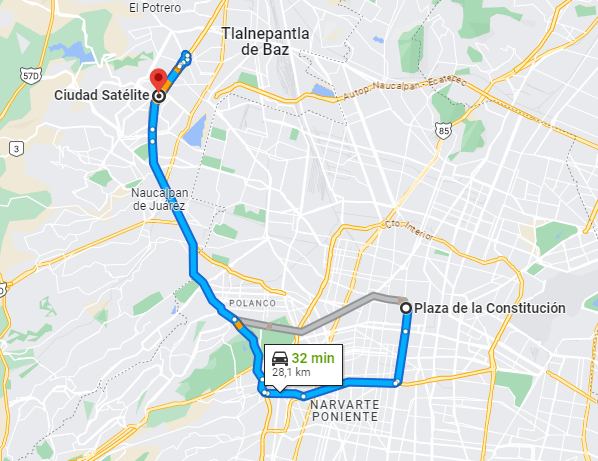
\includegraphics[scale=0.45]{Imagenes/Trayectoria_01.png}
    \caption{Ejemplo de una trayectoria.}
\end{figure}


Tipos de Trayectoria:

Cuando la trayectoria es una línea recta se dice que el movimiento es rectilíneo.

Cuando la trayectoria es un círculo decimos que el movimiento es circular.
\item El \textocolor{burgundy}{desplazamiento} de un móvil es una \textocolor{cerise}{magnitud vectorial}, ya que corresponde a una distancia medida en una dirección particular entre dos puntos: el de partida y el de llegada.

En el mismo ejemplo de ir del Zócalo de la CDMX a las Torres de Satélite, el desplazamiento se presenta como la línea que une los dos puntos.

Podemos tener distintas trayectorias, pero el desplazamiento entre dos puntos será siempre el mismo.
\begin{figure}[H]
    \centering
    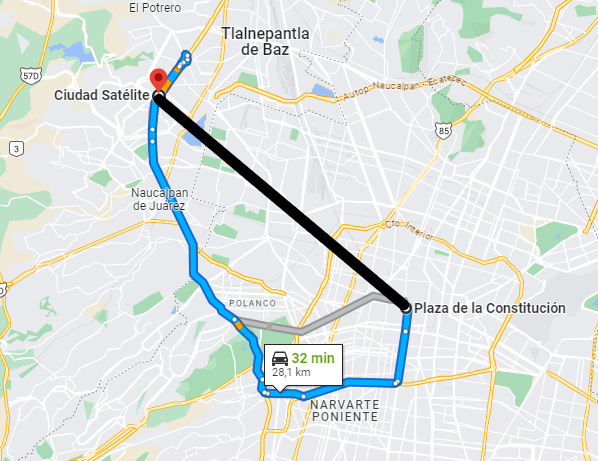
\includegraphics[scale=0.45]{Imagenes/Trayectoria_02.png}
    \caption{Desplazamiento entre dos puntos.}
\end{figure}
\end{enumerate}

\section{Movimiento Rectilíneo Uniforme.}

\subsection{Conceptos relevantes.}

\begin{enumerate}
\item La \textocolor{auburn}{rapidez} es la distancia recorrida por un objeto en cierto tiempo.

Es una \textocolor{awesome}{cantidad escalar}, porque se define con una magnitud y una unidad de medida.

La rapidez se obtiene mediante la siguiente expresión:
\begin{align*}
\text{rapidez} = \dfrac{\text{distancia}}{\text{tiempo}}
\end{align*}
Las unidades son metros por segundo (\unit[per-mode=symbol]{\meter\per\second})

\item La \textocolor{carmine}{velocidad} es la razón de cambio del desplazamiento de un objeto con respecto al tiempo.

La velocidad es una \textocolor{byzantine}{magnitud vectorial}.

La velocidad se obtiene mediante la siguiente expresión:
\begin{eqnarray*}
\begin{aligned}
\text{velocidad} = \dfrac{\text{desplazamiento}}{\text{tiempo}}  \hspace*{1.5cm} v = \dfrac{d}{t}
\end{aligned}
\end{eqnarray*}
Las unidades de la velocidad son metros por segundo (\unit[per-mode=symbol]{\meter\per\second})
\item La \textocolor{coolblack}{velocidad final} es el último instante o momento de la distancia recorrida en el tiempo.
\item La \textocolor{cornellred}{velocidad media} es el promedio de la suma de todas las distancias y tiempos recorridos.
\end{enumerate}

\subsection{El triángulo de la velocidad.}

En física es común apoyarse con ciertas reglas de tipo visual, que nos ayudarán a simplificar el manejo de una expresión.

Tal es el caso del \textbf{Triángulo de la velocidad}.

\begin{figure}[H]
\centering
\begin{tikzpicture}
    \draw (0, 0) -- (4, 0) -- (2, 2) -- cycle;
    \draw (2, 0) -- (2, 0.8);
    \draw (0.8, 0.8) -- (3.2, 0.8);

    \node at (2, 1.2) {$d$};
    \node at (1.2, 0.4) {$v$};
    \node at (2.8, 0.4) {$t$};
\end{tikzpicture}
\end{figure}
La idea con esta imagen es recuperar de la expresión, la operación que se necesite si nos piden alguna de las tres variables.

\subsection{Ejercicios de velocidad.}

\subsubsection{Ejercicio 1.}

Un corredor avanza \SI{2}{\kilo\meter} en un tiempo de \SI{15}{\minute}.

\vspace*{0.5cm}
Calcula su velocidad en \unit[per-mode=symbol]{\kilo\meter\per\hour} y en \unit[per-mode=symbol]{\meter\per\second}. Revisa que nos piden hacer una conversión de unidades.

\begin{enumerate}
\item Primer paso para la solución al ejercicio:

Se recomienda siempre tener los \textocolor{red}{DATOS} que nos indica el enunciado.
\begin{eqnarray*}
\begin{aligned}
\text{desplazamiento} &= \SI{2}{\kilo\meter} \\[0.5em] 
\text{tiempo} &= \SI{15}{\minute}
\end{aligned}
\end{eqnarray*}
\item Segundo paso para la solución al ejercicio:

Nos conviene anotar la \textocolor{red}{EXPRESIÓN} a utilizar, ya sea de uso directo o tengamos que despejar alguna variable.  Nos apoyamos con el triángulo de la velocidad:
\begin{minipage}{0.4\linewidth}
\begin{figure}[H]
\centering
\begin{tikzpicture}
    \draw (0, 0) -- (4, 0) -- (2, 2) -- cycle;
    \draw (2, 0) -- (2, 0.8);
    \draw (0.8, 0.8) -- (3.2, 0.8);

    \node at (2, 1.2) {$d$};
    \node at (1.2, 0.4) {$v$};
    \node at (2.8, 0.4) {$t$};
\end{tikzpicture}
\end{figure}
\end{minipage}
\hspace{0.5cm}
\begin{minipage}{0.4\linewidth}
\begin{align*}
v = \dfrac{d}{t}
\end{align*}
\end{minipage}
\item Tercer paso para la solución al ejercicio:

Hacemos la \textocolor{red}{SUSTITUCIÓN} con los valores que nos indica el enunciado:
\begin{eqnarray*}
\begin{aligned}
v = \dfrac{\SI{2}{\kilo\meter}}{\SI{15}{\minute}} =  \SI[per-mode=fraction]{0.1333}{\kilo\meter\per\minute}
\end{aligned}
\end{eqnarray*}
Tenemos la velocidad en \unit{\kilo\meter\per\minute}, pero nos piden se exprese en:
\begin{enumerate}[label=\alph*)]
\item Unidades de \unit{\kilo\meter\per\hour}

El factor de conversión es:
\begin{align*}
\SI{1}{\hour} = \SI{60}{\minute}
\end{align*}
Por lo que en la conversión se tiene:
\begin{eqnarray*}
\begin{aligned}
v &= \SI[per-mode=fraction]{0.1333}{\kilo\meter\per\minute} \left( \dfrac{\SI{60}{\minute}}{\SI{1}{\hour}} \right) =  \SI[per-mode=fraction]{8}{\kilo\meter\per\hour}
\end{aligned}
\end{eqnarray*}
\item Unidades de \unit{\meter\per\second}

Los factores de conversión son:
\begin{align*}
\SI{1}{\kilo\meter} &= \SI{1000}{\meter} \\[0.5em]
\SI{1}{\minute} &= \SI{60}{\second}
\end{align*}
Por lo que al utilizar los factores de conversión tenemos:
\begin{align*}
v &= \SI[per-mode=fraction]{0.1333}{\kilo\meter\per\minute} \left( \dfrac{\SI{1000}{\meter}}{\SI{1}{\kilo\meter}} \right) \left( \dfrac{\SI{1}{\minute}}{\SI{60}{\second}} \right)  =  \SI[per-mode=fraction]{2.22}{\meter\per\second}
\end{align*}
\end{enumerate}
\end{enumerate}

\subsubsection{Ejercicio 2.}

Un ciclista puede alcanzar en una bajada una velocidad de hasta \SI{35}{\kilo\meter\per\hour}.

¿Qué distancia recorre en una pendiente después de \SI{2}{\minute}?

\textocolor{red}{1. Datos} del enunciado:
\begin{eqnarray*}
\begin{aligned}
v &= \SI{35}{\kilo\meter\per\hour} \\[0.5em] 
t &= \SI{2}{\minute} \\[0.5em] 
d &= \, ? \, \text{ es la incógnita por resolver}
\end{aligned}
\end{eqnarray*}

\textocolor{red}{2. Expresión} a utilizar:

\begin{minipage}{0.4\linewidth}
\begin{figure}[H]
\centering
\begin{tikzpicture}
    \draw (0, 0) -- (4, 0) -- (2, 2) -- cycle;
    \draw (2, 0) -- (2, 0.8);
    \draw (0.8, 0.8) -- (3.2, 0.8);

    \node at (2, 1.2) {$d$};
    \node at (1.2, 0.4) {$v$};
    \node at (2.8, 0.4) {$t$};
\end{tikzpicture}
\end{figure}
\end{minipage}
\hspace{0.5cm}
\begin{minipage}{0.4\linewidth}
\begin{align*}
d = v \, t
\end{align*}
\end{minipage}

\vspace{0.5cm}
Conversión de unidades.

Antes de hacer la sustitución, debemos de hacer una conversión de unidades para mantener la congruencia con el resultado:

\begin{eqnarray*}
\begin{aligned}
\SI[per-mode=fraction]{35}{\kilo\meter\per\hour} \left( \dfrac{\SI{d3}{\meter}}{\SI{1}{\kilo\meter}} \right) \left( \dfrac{\SI{1}{\hour}}{\SI{60}{\minute}} \right) = \SI[per-mode=fraction]{583.3}{\meter\per\minute}
\end{aligned}
\end{eqnarray*}

\textocolor{red}{3. Sustitución} de los valores:
\begin{eqnarray*}
\begin{aligned}
d &= v \, t  = \left( \SI[per-mode=fraction]{583.3}{\meter\per\minute} \right) \left( \SI{2}{\minute} \right) = \\[0.5em] 
d &= \SI{1166.6}{\meter}
\end{aligned}
\end{eqnarray*}

\subsubsection{Ejercicio 3.}

Un auto viaja en una carretera a una velocidad constante de \SI{120}{\kilo\meter\per\hour}

\vspace*{0.3cm}
¿Cuánto tiempo le tomará llegar al poblado más cercano, que está a \SI{180}{\kilo\meter} a esa misma velocidad?

\vspace*{0.3cm}
\begin{minipage}[t]{0.4\linewidth}
\textocolor{red}{1. Datos:}
\begin{align*}
v &= \SI{120}{\kilo\meter\per\hour} \\[0.5em]
d &= \SI{180}{\kilo\meter} \\[0.5em]
t &= \, ?
\end{align*}
\end{minipage}
\hspace{0.5cm}
\begin{minipage}[t]{0.4\linewidth}
\textocolor{red}{2. Expresión:}
\begin{eqnarray*}
\begin{aligned}
v = \dfrac{d}{t} \hspace{0.3cm} \Rightarrow \hspace{0.3cm} t = \dfrac{d}{v}
\end{aligned}
\end{eqnarray*}
\end{minipage}

\newpage
\textocolor{red}{3. Sustitución:}

Una vez conocida la expresión que debemos de ocupar, procedemos a sustituir los valores que nos indica el enunciado.
\begin{align*}
t = \dfrac{\SI{180}{\kilo\meter}}{\SI{120}{\kilo\meter\per\hour}} =  \SI{1.5}{\hour}
\end{align*}

\section{Interpretando una gráfica.}

El movimiento de un cuerpo se puede representar de manera oportuna mediante una gráfica,  por lo que será conveniente revisar la manera en la que podemos \enquote{leer} la información contenida en esa gráfica.

Comenzamos reconociendo que en el \textocolor{cadetblue}{eje de las abscisas} (el eje horizontal, también conocido como el eje de las $x$) tendremos siempre la \textocolor{magenta}{variable temporal}, es decir, el tiempo $t$. El tiempo será la \textocolor{alizarin}{variable independiente}.

En el \textocolor{ballblue}{eje de las ordenadas} (que es el eje vertical, conocido como el eje de las $y$), tendremos la variable de \textocolor{auburn}{desplazamiento}, que representamos por $d$. El desplazamiento será la \textocolor{burntumber}{variabe dependiente}.

\begin{figure}[H]
    \centering
    \begin{tikzpicture}[scale=1]
        \draw (0, 0) -- (7.5, 0) node [above, pos=1] {\small{$t \, [\unit{\second}]$}};
        \draw (0, 0) -- (0, 5.3) node [left, pos=1.1] {\small{$d \, [\unit{\meter}]$}};
    \end{tikzpicture}
    \caption{Sistema coordenado para graficar la distancia contra el tiempo}
\end{figure}

\subsection{La recta.}

Para estudiar el \textocolor{byzantium}{Movimiento Rectilíneo Uniforme}, es necesario recordar la recta y su ecuación. Sabemos desde los griegos que para trazar un recta se necesitan al menos dos puntos, llamemos a esos puntos $(x_{i}, y_{i})$ y $(x_{f}, y_{f})$.

Donde:
\begin{enumerate}[label=\alph*)]
\item $x_{i}$ es el tiempo inicial donde comienza el desplazamiento.
\item $x_{f}$ es el tiempo final donde termina el desplazamiento del objeto.
\item $y_{i}$ es el desplazamiento inicial del objeto.
\item $y_{f}$ es el desplazamiento final del objeto.
\end{enumerate} 

\begin{figure}[H]
    \centering
    \begin{tikzpicture}[scale=0.9]
        \draw (0, 0) -- (7.5, 0) node [above, pos=1] {\small{$t \, [\unit{\second}]$}};
        \draw (0, 0) -- (0, 5.3) node [left, pos=1.1] {\small{$d \, [\unit{\meter}]$}};

        \draw (1, 2.3) node {$+$};
        \node at (2, 2.3) {\small{$(x_{i}, y_{i})$}};
        
        \draw [dashed] (1, 0) -- (1, 2.3);
        \node at (1, -0.3) {\small{$x_{i}$}};
        \draw [dashed] (0, 2.3) -- (1, 2.3);
        \node at (-0.6, 2.3) {\small{$y_{i}$}};
        
        
        \draw (4.5, 4.5) node {$+$};
        \node at (5.9, 4.5) {\small{$(x_{f}, y_{f})$}};
        
        \draw [dashed] (4.5, 0) -- (4.5, 4.5);
        \node at (4.5, -0.3) {\small{$x_{f}$}};
        \draw [dashed] (0, 4.5) -- (4.5, 4.5);
        \node at (-0.6, 4.5) {\small{$y_{f}$}};
    \end{tikzpicture}
    \caption{Dos puntos que representan el desplazamiento de un objeto en un intervalo de tiempo.}
\end{figure}

Con los dos puntos anteriores, podemos trazar una recta que pase por esos puntos.
\begin{figure}[H]
    \centering
    \begin{tikzpicture}[scale=1]
        \draw (0, 0) -- (7.5, 0) node [above, pos=1] {\small{$t \, [\unit{\second}]$}};
        \draw (0, 0) -- (0, 5.3) node [left, pos=1.1] {\small{$d \, [\unit{\meter}]$}};

        \draw (1, 2.45) node {$+$};
        \node at (1, 1.7) {\small{$(x_{i}, y_{i})$}};

        \draw (4.5, 4.32) node {$+$};
        \node at (5.9, 4.5) {\small{$(x_{f}, y_{f})$}};
        
        \draw [thick, color=ao] (1, 2.45) -- (4.5, 4.32);

        % \draw [dashed] (1, 2.45) -- (4.5, 2.45);
        % \node at (2.7, 2) {\small{$\Delta x$}};
        % \draw [dashed] (4.5, 4.32) -- (4.5, 2.45);
        % \node at (4.9, 3.5) {\small{$\Delta y$}};

        % \node at (6.5, 2.5) {\small{$m = \dfrac{\Delta y}{\Delta x}$}};
    \end{tikzpicture}
    \caption{Recta que pasa por los dos puntos.}
\end{figure}

Para obtener una cantidad importante de la recta, necesitamos medir el cambio tanto en el eje horizontal como en el eje vertical, para ello denotamos como $\Delta x$ el cambio en el eje de las abscisas, mientras que $\Delta y$ es el cambio en el eje de las ordenadas.
\begin{figure}[H]
    \centering
    \begin{tikzpicture}[scale=1]
        \draw (0, 0) -- (7.5, 0) node [above, pos=1] {\small{$t \, [\unit{\second}]$}};
        \draw (0, 0) -- (0, 5.3) node [left, pos=1.1] {\small{$d \, [\unit{\meter}]$}};

        \draw (1, 2.45) node {$+$};
        \node at (1, 1.7) {\small{$(x_{i}, y_{i})$}};

        \draw (4.5, 4.32) node {$+$};
        \node at (5.9, 4.5) {\small{$(x_{f}, y_{f})$}};
        
        \draw [thick, color=ao] (1, 2.45) -- (4.5, 4.32);

        \draw [dashed] (1, 2.45) -- (4.5, 2.45);
        \node at (2.7, 2) {\small{$\Delta x$}};
        \draw [dashed] (4.5, 4.32) -- (4.5, 2.45);
        \node at (4.9, 3.5) {\small{$\Delta y$}};

        % \node at (6.5, 2.5) {\small{$m = \dfrac{\Delta y}{\Delta x}$}};
    \end{tikzpicture}
    \caption{Cambios en los ejes horizontal y vertical.}
\end{figure}

De la misma geometría sabemos que la pendiente de una recta es la cantidad:
\begin{align*}
m = \dfrac{\Delta y}{\Delta x} =  \dfrac{y_{f} - y_{i}}{x_{f} - x_{i}}
\end{align*}
\begin{figure}[H]
    \centering
    \begin{tikzpicture}[scale=1]
        \draw (0, 0) -- (7.5, 0) node [above, pos=1] {\small{$t \, [\unit{\second}]$}};
        \draw (0, 0) -- (0, 5.3) node [left, pos=1.1] {\small{$d \, [\unit{\meter}]$}};

        \draw (1, 2.45) node {$+$};
        \node at (1, 1.7) {\small{$(x_{i}, y_{i})$}};

        \draw (4.5, 4.32) node {$+$};
        \node at (5.9, 4.5) {\small{$(x_{f}, y_{f})$}};
        
        \draw [thick, color=ao] (1, 2.45) -- (4.5, 4.32);

        \draw [dashed] (1, 2.45) -- (4.5, 2.45);
        \node at (2.7, 2) {\small{$\Delta x$}};
        \draw [dashed] (4.5, 4.32) -- (4.5, 2.45);
        \node at (4.9, 3.5) {\small{$\Delta y$}};

        \node at (6.5, 2.5) {\small{$m = \dfrac{\Delta y}{\Delta x}$}};
    \end{tikzpicture}
    \caption{Pendiente de la recta.}
\end{figure}

Como estamos estudiando el desplazamiento de un objeto con respecto al tiempo, en la gráfica de d vs t, la pendiente de la recta es la \textocolor{cobalt}{velocidad} del objeto.

En algunos casos, podemos tomar el valor inicial en el eje vertical, es decir, el eje $y$, en este caso, decimos que la ordenada al origen $b$ representa la posición inicial del objeto antes de que comience el movimiento.
\begin{figure}[H]
    \centering
    \begin{tikzpicture}[scale=0.9]
        \draw (0, 0) -- (7.5, 0) node [above, pos=1] {\small{$t \, [\unit{\second}]$}};
        \draw (0, 0) -- (0, 5.3) node [left, pos=1.1] {\small{$d \, [\unit{\meter}]$}};

        \draw (1, 2.45) node {$+$};
        \node at (1, 1.7) {\small{$(x_{i}, y_{i})$}};
        
        \draw (4.5, 4.32) node {$+$};
        \node at (5.9, 4.5) {\small{$(x_{f}, y_{f})$}};
                
        \draw [thick, color=ao] (0, 2) -- (5, 4.5);

        \node at (-0.4, 2) {\small{$b$}};
    \end{tikzpicture}
\end{figure}

\subsection{La ecuación de la recta.}

La expresión completa para la ecuación de una recta es:
\begin{align*}
y = m \, x + b
\end{align*}
donde $m$ representa la pendiente y $b$ la ordenada en el origen.

\subsection{Signo de la pendiente.}

\begin{enumerate}
\item El primer caso a revisar es cuando la pendiente de la recta vale $0$, es decir, cuando es paralela al eje horizontal.
\begin{figure}[H]
    \centering
    \begin{tikzpicture}[scale=0.9]
        \draw (0, 0) -- (7.5, 0) node [above, pos=1] {\small{$t \, [\unit{\second}]$}};
        \draw (0, 0) -- (0, 5.3) node [left, pos=1.1] {\small{$d \, [\unit{\meter}]$}};

        \foreach [evaluate={\j=int(\x*10)}] \x in {1, 2, 3, 4, 5, 6, 7}
        {    
            \draw (\x, 0.2) -- (\x, -0.2);
            \node at (\x, -0.4) {\small{$\x$}};
        }
        \foreach [evaluate={\j=int(\x*10)}] \x in {1, 2, 3, 4, 5}
        {
            \draw (-0.2, \x) -- (0.2, \x);
            \node at (-0.6, \x) {\small{$\j$}};
        }
        
        \draw [thick, color=ao] (0, 4) -- (7, 4); 
    \end{tikzpicture}
    \caption{Caso de la pendiente con valor cero.}
\end{figure}
De la gráfica anterior vemos que conforme transcurre el tiempo (en el eje horizontal), el objeto no cambia de posición, ocupando la expresión que revisamos anteriormente:
\begin{align*}
m = \dfrac{\Delta y}{\Delta x} =  \dfrac{\SI{40}{\meter} - \SI{40}{\meter}}{t} = 0
\end{align*}
Por lo tanto, la velocidad del objeto es cero, el objeto permanece en \textocolor{crimsonglory}{reposo}.

\item La pendiente con \textocolor{cadmiumgreen}{valor positivo}, indica que el objeto \textocolor{cadmiumgreen}{incrementa su velocidad}.
\begin{figure}[H]
    \centering
    \begin{tikzpicture}[scale=0.9]
        \draw (0, 0) -- (7.5, 0) node [above, pos=1] {\small{$t \, [\unit{\second}]$}};
        \draw (0, 0) -- (0, 5.3) node [left, pos=1.1] {\small{$d \, [\unit{\meter}]$}};

        \draw [thick, color=ao] (0, 2) -- (5, 4.5);
    \end{tikzpicture}
    \caption{Ejemplo de una recta con pendiente positiva.}
\end{figure}
\item La pendiente con \textocolor{carmine}{valor negativo}, nos dice que el objeto \textocolor{carmine}{disminuye su velocidad}.
\begin{figure}[H]
    \centering
    \begin{tikzpicture}[scale=0.9]
        \draw (0, 0) -- (7.5, 0) node [above, pos=1] {\small{$t \, [\unit{\second}]$}};
        \draw (0, 0) -- (0, 5.3) node [left, pos=1.1] {\small{$d \, [\unit{\meter}]$}};

        \draw [thick, color=ao] (1, 4.5) -- (5, 1);
    \end{tikzpicture}
    \caption{Ejemplo de una recta con pendiente negativa.}
\end{figure}
\end{enumerate}

\subsection{La ordenada al origen.}

Ya se mencionó que la ordenada al origen $b$, en una gráfica de $d$ vs. $t$ representa la posición inicial del objeto, hay que considerar entonces que este valor puede tomar tres casos.

\begin{enumerate}[label=\alph*)]
\item $\mathbf{b = 0}$.

En este caso, interpretamos que la posición del objeto coincide con el origen de nuestro sistema coordenado: al tiempo inicial, se encuentra en el origen de nuestro eje $y$.
\begin{figure}[H]
    \centering
    \begin{tikzpicture}[scale=1]
        \draw (0, 0) -- (4.5, 0) node [above, pos=1] {\small{$t \, [\unit{\second}]$}};
        \draw (0, 0) -- (0, 4.5) node [left, pos=1.1] {\small{$d \, [\unit{\meter}]$}};

        \draw [thick, color=ao] (0, 0) -- (4, 4);
    \end{tikzpicture}
    \caption{Ordenada en el origen $b = 0$}
\end{figure}
\item $\mathbf{b > 0}$.

El objeto se encuentra desplazado una distancia positiva por arriba del origen, pensemos como ejemplo que en un maratón, un corredor al momento del disparo de arranque se encuentra adelante del punto inicial.
\begin{figure}[H]
    \centering
    \begin{tikzpicture}[scale=1]
        \draw (0, 0) -- (4.5, 0) node [above, pos=1] {\small{$t \, [\unit{\second}]$}};
        \draw (0, 0) -- (0, 4.5) node [left, pos=1.1] {\small{$d \, [\unit{\meter}]$}};

        \draw [thick, color=ao] (0, 2) -- (4, 4);
    \end{tikzpicture}
    \caption{Ordenada en el origen $b > 0$}
\end{figure}
\item $\mathbf{b < 0}$.

El objeto se encuentra desplazado una distancia negativa por debajo del origen, en el mismo ejemplo del maratón, ahora el corredor al momento del disparo de arranque se encuentra atrás del punto inicial.
\begin{figure}[H]
    \centering
    \begin{tikzpicture}[scale=1]
        \draw (0, 0) -- (4, 0) node [above, pos=1] {\small{$t \, [\unit{\second}]$}};
        \draw (0, -1.5) -- (0, 3) node [left, pos=1.1] {\small{$d \, [\unit{\meter}]$}};

        \draw [thick, color=ao] (0, -1) -- (3, 3);
    \end{tikzpicture}
    \caption{Ordenada en el origen $b < 0$}
\end{figure}
\end{enumerate}

\subsection{Estudiando una gráfica.}

El siguiente paso es estudiar una gráfica de desplazamiento contra tiempo, haciéndolo por intervalos de tiempo.


Por ejemplo: Determina la velocidad del objeto en los intervalos de tiempo que se muestran en la siguiente gráfica.

\begin{enumerate}[label=\roman*)]
\item De $0$ a $1$ segundo.
\item De $1$ a $3$ segundos.
\item De $3$ a $4$ segundos.
\item De $4$ a $5$ segundos.
\item De $5$ a $7$ segundos.
\end{enumerate}

\begin{figure}[H]
    \centering
    \begin{tikzpicture}
        \draw (0, 0) -- (7.5, 0) node [above, pos=1] {\small{$t \, [\unit{\second}]$}};
        \draw (0, 0) -- (0, 5.3) node [left, pos=1.1] {\small{$d \, [\unit{\meter}]$}};

        \foreach [evaluate={\j=int(\x*10)}] \x in {1, 2, 3, 4, 5, 6, 7}
        {    
            \draw (\x, 0.2) -- (\x, -0.2);
            \node at (\x, -0.4) {\small{$\x$}};
        }
        \foreach [evaluate={\j=int(\x*10)}] \x in {1, 2, 3, 4, 5}
        {
            \draw (-0.2, \x) -- (0.2, \x);
            \node at (-0.6, \x) {\small{$\j$}};
        }
        
        \draw [thick, color=ao] (0, 0) -- (1, 1); 
        \draw [thick, color=ao] (1, 1) -- (3, 2); 
        \draw [thick, color=ao] (3, 2) -- (4, 4); 
        \draw [thick, color=ao] (4, 4) -- (5, 5); 
        \draw [thick, color=ao] (5, 5) -- (7, 5); 
    \end{tikzpicture}
\end{figure}

Para resolver este ejercicio, debemos de ocupar la expresión para la velocidad pero en términos de los puntos que definen cada segmento de recta:
\begin{align*}
v = \dfrac{\Delta y}{\Delta x} = \dfrac{y_{f} - y_{1}}{x_{f} - x_{i}}
\end{align*}
Por lo que tendremos:
\begin{enumerate}[label=\roman*)]
\item De $0$ a $1$ segundo.
\begin{align*}
v = \dfrac{y_{f} - y_{1}}{x_{f} - x_{i}} = \dfrac{\SI{10}{\meter} - \SI{0}{\meter}}{\SI{1}{\second} - \SI{0}{\second}} = \dfrac{\SI{10}{\meter}}{\SI{1}{\second}} = \SI[per-mode=fraction]{10}{\meter\per\second}
\end{align*}
\item De $1$ a $3$ segundos.
\begin{align*}
v = \dfrac{y_{f} - y_{1}}{x_{f} - x_{i}} = \dfrac{\SI{20}{\meter} - \SI{10}{\meter}}{\SI{3}{\second} - \SI{1}{\second}} = \dfrac{\SI{10}{\meter}}{\SI{2}{\second}} = \SI[per-mode=fraction]{5}{\meter\per\second}
\end{align*}
\item De $3$ a $4$ segundos.
\begin{align*}
v = \dfrac{y_{f} - y_{1}}{x_{f} - x_{i}} = \dfrac{\SI{40}{\meter} - \SI{20}{\meter}}{\SI{4}{\second} - \SI{3}{\second}} = \dfrac{\SI{20}{\meter}}{\SI{1}{\second}} = \SI[per-mode=fraction]{20}{\meter\per\second}
\end{align*}
\item De $4$ a $5$ segundos.
\begin{align*}
v = \dfrac{y_{f} - y_{1}}{x_{f} - x_{i}} = \dfrac{\SI{50}{\meter} - \SI{40}{\meter}}{\SI{5}{\second} - \SI{4}{\second}} = \dfrac{\SI{10}{\meter}}{\SI{1}{\second}} = \SI[per-mode=fraction]{10}{\meter\per\second}
\end{align*}
\item De $5$ a $7$ segundos.
\begin{align*}
v = \dfrac{y_{f} - y_{1}}{x_{f} - x_{i}} = \dfrac{\SI{50}{\meter} - \SI{50}{\meter}}{\SI{7}{\second} - \SI{5}{\second}} = \dfrac{\SI{0}{\meter}}{\SI{2}{\second}} = \SI[per-mode=fraction]{0}{\meter\per\second}
\end{align*}
En este intervalo el objeto permanece en reposo, está ubicado a \SI{50}{\meter} del origen.
\end{enumerate}

\section{Movimiento uniformemente acelerado.}

\subsection{La aceleración.}

Supongamos que un cuerpo se mueve a lo largo de una línea recta y cada segundo se registra que su velocidad aumenta (o disminuye) en \SI{10}{\meter\per\second}.

De manera que al tiempo incial $t = 0$, la velocidad es v = \SI{0}{\meter\per\second}, es decir, al inicio del movimiento, el objeto parte con velocidad cero, al segundo $1$ su velocidad es de \SI{10}{\meter\per\second},  al segundo $2$ es de \SI{20}{\meter\per\second},  al segundo $3$ es \SI{30}{\meter\per\second},  al segundo $4$ es \SI{40}{\meter\per\second},  y por último al segundo $5$, su velocidad es \SI{50}{\meter\per\second}.
\begin{table}[H]
\renewcommand{\arraystretch}{1}
\centering
\begin{tabular}{c | c}
Tiempo [\unit{\second}] & Velocidad [\unit{\meter\per\second}] \\ \hline
$0$ & $0$ \\ \hline
$1$ & $10$ \\ \hline
$2$ & $20$ \\ \hline
$3$ & $30$ \\ \hline
$4$ & $40$ \\ \hline
$5$ & $50$ \\ \hline
\end{tabular}
\end{table}

Al graficar el conjunto de datos de la tabla anterior, en un sistema coordenado donde el eje vertical corresponde para la velocidad $v$ y en el eje horizontal corresponde para el tiempo, tendremos la siguiente figura:
\begin{figure}[H]
    \centering
    \begin{tikzpicture}
        \draw (0, 0) -- (6, 0) node [above, pos=1] {\small{$t \, [\unit{\second}]$}};
        \draw (0, 0) -- (0, 5.3) node [left, pos=1.1] {\small{$v \, [\unit{\meter\per\second}]$}};

        \foreach [evaluate={\j=int(\x*10)}] \x in {1, 2, 3, 4, 5}
            {    
            \draw (\x, 0.2) -- (\x, -0.2);
            \node at (\x, -0.4) {\small{$\x$}};

            \draw (-0.2, \x) -- (0.2, \x);
            \node at (-0.6, \x) {\small{$\j$}};
            }

            \foreach \x in {0, 1, 2, 3, 4, 5}
                {
                    \draw [color=blue, fill] (\x, \x) circle (0.4mm);
                    \draw [dashed] (\x, 0) -- (\x, \x);
                    \draw [dashed] (0, \x) -- (\x, \x); 
                }
    \end{tikzpicture}
\end{figure}

Al tener varios puntos en la gráfica, podemos trazar una recta por los mismos.
\begin{figure}[H]
    \centering
    \begin{tikzpicture}
        \draw (0, 0) -- (6, 0) node [above, pos=1] {\small{$t \, [\unit{\second}]$}};
        \draw (0, 0) -- (0, 5.3) node [left, pos=1.1] {\small{$v \, [\unit{\meter\per\second}]$}};

        \foreach [evaluate={\j=int(\x*10)}] \x in {1, 2, 3, 4, 5}
            {    
            \draw (\x, 0.2) -- (\x, -0.2);
            \node at (\x, -0.4) {\small{$\x$}};

            \draw (-0.2, \x) -- (0.2, \x);
            \node at (-0.6, \x) {\small{$\j$}};
            }

        \foreach \x in {0, 1, 2, 3, 4, 5}
            \draw [color=blue, fill] (\x, \x) circle (0.4mm);

        \draw [thick, red] (0, 0) -- (5, 5);

    \end{tikzpicture}
\end{figure}

Con estos datos reconocemos que la velocidad está variando en \SI{10}{\meter\per\second} cada \SI{1}{\second}, esto es, el cuerpo tiene una aceleración de \SI{10}{\meter\per\square\second}.

Definimos la \textocolor{red}{aceleración} como la razón de cambio de la velocidad $(\Delta v)$ con respecto al tiempo $(\Delta t)$, siendo una \textocolor{cerise}{cantidad vectorial}, porque consta de un magnitud o valor, dirección y sentido.

Al igual que con la velocidad, es posible presentar una expresión para la aceleración:
\begin{align*}
a &= \dfrac{\text{cambio de velocidad}}{\text{intervalo de tiempo}} =  \dfrac{\Delta \, v}{\Delta \, t} = \\[1em] 
a &= \dfrac{\text{Velocidad final - Velocidad inicial}}{\text{tiempo}} = \\[1em] 
a &= \dfrac{v_{f} - v_{i}}{t}
\end{align*}
donde:
\begin{enumerate}[label=\roman*)]
\item La \textocolor{cobalt}{velocidad inicial} ($v_{i}$) del objeto se define como la velocidad del móvil al inicio del intervalo de tiempo, y que si el objeto se encuentra \textocolor{byzantine}{en reposo}, esta velocidad tiene un valor de cero.
\item La \textocolor{bole}{velocidad final} ($v_{f}$) se define como la velocidad al terminar el intervalo de tiempo.
\end{enumerate}
En la gráfica anterior donde tenemos en el eje vertical a la velocidad $v$, y en el eje horizontal al tiempo $t$, reconocemos ahora que la pendiente de la recta es la aceleración.

También como con la velocidad, estudiando la pendiente de la recta, tendremos lo siguiente:
\begin{enumerate}[label=\alph*)]
\item Se considera que un móvil tiene una \textocolor{darkgreen}{aceleración positiva}  cuando \textocolor{darkgreen}{aumenta} su velocidad.

En la gráfica de $v$ vd $t$, la \textocolor{coquelicot}{pendiente de la recta es positiva}.
\item Si \textocolor{blue-violet}{disminuye su velocidad} tiene \textocolor{blue-violet}{aceleración negativa} (conocida también como desaceleración o frenado), el valor de la aceleración lleva un signo negativo.

En una gráfica de $v$ vd $t$, la \textocolor{awesome}{pendiente de la recta es negativa}.
\item De igual modo se considera que un cuerpo no tiene aceleración ($a = 0$)  si \textocolor{cerise}{está inmóvil} o si se mueve con \textocolor{bulgarianrose}{velocidad constante}.

En una gráfica de $v$ vd $t$, la \textocolor{cadetblue!60!black}{pendiente de la recta es cero}.
\end{enumerate}

\subsection{Ejercicios de aceleración.}

\subsubsection{Enunciado del ejercicio 1.}

Un autobús viaja en una carretera a una velocidad de \SI{70}{\kilo\meter\per\hour} y acelera durante \SI{30}{\second} hasta llegar a su límite de velocidad, que son \SI{95}{\kilo\meter\per\hour}.

¿Cuál fue su aceleración?

\vspace*{0.3cm}
Resolviendo el ejercicio 1:

\vspace*{0.3cm}
\begin{minipage}[t]{0.4\linewidth}
\textocolor{red}{1. Datos:}
\begin{align*}
v_{i} &= \SI{70}{\kilo\meter\per\hour} \\[0.5em] 
v_{f} &= \SI{95}{\kilo\meter\per\hour} \\[0.5em] 
t &= \SI{30}{\second} \\[0.5em] 
a &= \, ?
\end{align*}
\end{minipage}
\hspace{0.5cm}
\begin{minipage}[t]{0.4\linewidth}
\textocolor{red}{2. Expresión:}
\begin{align*}
a = \dfrac{v_{f} - v_{i}}{t}
\end{align*}
\end{minipage}

\vspace*{0.3cm}
Conversión de unidades: antes de sustituir, ajustamos las unidades de velocidad (recuerda que es importante manejar las correspondiente unidades del Sistema Internacional, para el caso de la velocidad, las unidades son \unit{\meter\per\second}):

\begin{align*}
v_{i} &= \left( \SI[per-mode=fraction]{70}{\kilo\meter\per\hour} \right)  \left( \dfrac{\SI{1000}{\meter}}{\SI{1}{\kilo\meter}} \right)  \left( \dfrac{\SI{1}{\hour}}{\SI{3600}{\second}} \right) = \SI[per-mode=fraction]{19.44}{\meter\per\second} \\[0.5em] 
v_{f} &= \left( \SI[per-mode=fraction]{95}{\kilo\meter\per\hour} \right)  \left( \dfrac{\SI{1000}{\meter}}{\SI{1}{\kilo\meter}} \right)  \left( \dfrac{\SI{1}{\hour}}{\SI{3600}{\second}} \right) = \SI[per-mode=fraction]{26.38}{\meter\per\second}
\end{align*}

\textocolor{red}{3. Sustitución:}
\begin{align*}
a &= \dfrac{ \displaystyle \SI[per-mode=fraction]{26.38}{\meter\per\second} - \SI[per-mode=fraction]{19.44}{\meter\per\second}}{\SI{30}{\second}} = \\[0.5em] 
a &= \dfrac{ \displaystyle \SI[per-mode=fraction]{6.94}{\meter\per\second}}{\SI{30}{\second}} = \\[0.5em] 
a &= \SI{0.2313}{\meter\per\square\second}
\end{align*}

\subsubsection{Enunciado del ejercicio 2.}

¿Qué tiempo le toma a un auto detenerse si iba a \SI{90}{\kilo\meter\per\hour} antes de aplicar los frenos y desacelerar a \SI{4}{\meter\per\square\second}?

Considera que en física hay que se muy cuidadosos al momento de leer el enunciado, ya que aunque no lo dice expresamente, la velocidad inicial del auto es $v_{i} = \SI{0}{\meter\per\second}$

\vspace{0.3cm}
\begin{minipage}[t]{0.4\linewidth}
\textocolor{red}{1. Datos:}
\begin{align*}
v_{i} &= \SI{90}{\kilo\meter\per\hour} \\[0.5em] 
v_{f} &= \SI{0}{\kilo\meter\per\hour} \\[0.5em] 
a &= - \SI{4}{\meter\per\square\second} \\[0.5em] 
t &= \, ?
\end{align*}
\end{minipage}
\hspace{0.5cm}
\begin{minipage}[t]{0.4\linewidth}
\textocolor{red}{2. Expresión:}
\begin{align*}
a &= \dfrac{v_{f} - v_{i}}{t} \\[0.5em] 
t &=  \dfrac{v_{f} - v_{i}}{a}
\end{align*}
\end{minipage}

\vspace{0.3cm}
Conversión de unidades: antes de sustituir, ajustamos las unidades de velocidad:
\begin{align*}
v_{i} &= \left( \SI[per-mode=fraction]{90}{\kilo\meter\per\hour} \right)  \left( \dfrac{\SI{1000}{\meter}}{\SI{1}{\kilo\meter}} \right)  \left( \dfrac{\SI{1}{\hour}}{\SI{3600}{\second}} \right) =  \SI[per-mode=fraction]{25}{\meter\per\second}
\end{align*}

\textocolor{red}{3. Sustitución:}
\begin{align*}
t &=  \dfrac{ \SI{0}{\meter\per\second} - \SI{25}{\meter\per\second}}{- \SI{4}{\meter\per\square\second}} = \dfrac{- \SI{25}{\meter\per\second}}{- \SI{4}{\meter\per\square\second}} = \SI{6.25}{\second}
\end{align*}

Que es la respuesta pedida, el auto se detendrá a los \SI{6.25}{\second} al desacelerar cuando se pisaron los frenos.

\subsection{Leyendo una gráfica de velocidad vs tiempo.}

Encontraremos la representación gráfica de la velocidad $v$ de un objeto contra el tiempo $t$, que al igual en el caso de la gráfica de $d$ vs $t$, las propiedades de la recta nos serán de utilidad.

Calcula la aceleración en cada segmento de la siguiente gráfica.
\begin{figure}[H]
    \centering
    \begin{tikzpicture}
        \draw (0, 0) -- (9, 0) node [above, pos=1.1] {\small{$t \, [\unit{\second}]$}};
        \draw (0, 0) -- (0, 5.3) node [left, pos=1.1] {\small{$v \, [\unit{\meter\per\second}]$}};

        \foreach \x in {1, 2,...,9}
            {    
            \draw (\x, 0.2) -- (\x, -0.2);
            \node at (\x, -0.4) {\small{$\x$}};
            }
        \foreach [evaluate={\j=int(\x*10)}] \x in {1, 2, 3, 4, 5}
            {
            \draw (-0.2, \x) -- (0.2, \x);
            \node at (-0.6, \x) {\small{$\j$}};
            }

        \draw [thick, color=blue-violet] (0, 0) -- (2, 2);
        \node at (-0.3, 0.1)  {\small{$A$}};

        \draw [thick, color=blue-violet] (2, 2) -- (4, 2);
        \node at (2, 2.2)  {\small{$B$}};

        \draw [thick, color=blue-violet] (4, 2) -- (6, 5);
        \node at (4, 1.8)  {\small{$C$}};

        \draw [thick, color=blue-violet] (6, 5) -- (9, 0);
        \node at (6, 5.2)  {\small{$D$}};

        \node at (9.2, 0.2)  {\small{$E$}};
    \end{tikzpicture}
\end{figure}

Ocuparemos la expresión que nos determina la aceleración a partir de un conjunto de puntos:
\begin{align*}
a = \dfrac{\Delta y}{\Delta x} = \dfrac{v_{f} - v_{i}}{t_{f} - t_{i}}
\end{align*}

Tendremos entonces que:
\begin{itemize}
\item En el segmento $A - B$:
\begin{align*}
a = \dfrac{\Delta y}{\Delta x} = \dfrac{v_{f} - v_{i}}{t_{f} - t_{i}} = \dfrac{\displaystyle \SI[per-mode=fraction]{20}{\meter\per\second} - \SI[per-mode=fraction]{0}{\meter\per\second}}{\SI{2}{\second} - \SI{0}{\second}} = \dfrac{ \displaystyle \SI[per-mode=fraction]{20}{\meter\per\second}}{\SI{2}{\second}} = \SI[per-mode=fraction]{10}{\meter\per\square\second}
\end{align*}
Vemos que la pendiente del segmento de recta es positivo.
\item En el segmento $B - C$:
\begin{align*}
a = \dfrac{\Delta y}{\Delta x} = \dfrac{v_{f} - v_{i}}{t_{f} - t_{i}} = \dfrac{\displaystyle \SI[per-mode=fraction]{20}{\meter\per\second} - \SI[per-mode=fraction]{20}{\meter\per\second}}{\SI{4}{\second} - \SI{2}{\second}} = \dfrac{ \displaystyle \SI[per-mode=fraction]{0}{\meter\per\second}}{\SI{2}{\second}} = \SI[per-mode=fraction]{0}{\meter\per\square\second}
\end{align*}
En este intervalo la aceleración es cero, pero revisa que el objeto se desplaza a una velocidad constante de \SI{20}{\meter\per\second}, es un ejemplo en donde a pesar de que el objeto se está moviendo, no tiene aceleración. La pendiente del segmento de recta es paralela al eje horizontal, por lo que la pendiente vale cero.
\item En el segmento $C- D$:
\begin{align*}
a = \dfrac{\Delta y}{\Delta x} = \dfrac{v_{f} - v_{i}}{t_{f} - t_{i}} = \dfrac{\displaystyle \SI[per-mode=fraction]{50}{\meter\per\second} - \SI[per-mode=fraction]{20}{\meter\per\second}}{\SI{6}{\second} - \SI{4}{\second}} = \dfrac{ \displaystyle \SI[per-mode=fraction]{30}{\meter\per\second}}{\SI{2}{\second}} = \SI[per-mode=fraction]{15}{\meter\per\square\second}
\end{align*}
\item En el segmento $D - E$:
\begin{align*}
a = \dfrac{\Delta y}{\Delta x} = \dfrac{v_{f} - v_{i}}{t_{f} - t_{i}} = \dfrac{\displaystyle \SI[per-mode=fraction]{0}{\meter\per\second} - \SI[per-mode=fraction]{50}{\meter\per\second}}{\SI{9}{\second} - \SI{6}{\second}} = \dfrac{ \displaystyle - \SI[per-mode=fraction]{50}{\meter\per\second}}{\SI{3}{\second}} = - \SI[per-mode=fraction]{16.66}{\meter\per\square\second}
\end{align*}
Se tiene que la pendiente de la recta es negativa, por lo tanto en este segmento de recta el objeto se está desacelerando hasta llegar a una velocidad cero, en este caso, el objeto queda en reposo.
\end{itemize}
Revisa que en cada operación de sustitución \textbf{se han usasdo las unidades correspondientes}, de esta manera estamos escribiendo debidamente las expresiones en física, si omitimos las unidades, solo estamos haciendo operaciones aritméticas, no física.



\end{document}